\documentclass[xcolor=table]{beamer}

\usepackage{lscape, amsmath, amsfonts, amssymb, setspace, theorem, wrapfig, graphicx, float, multirow, subfig, color, rotating, multicol, datetime, natbib, venndiagram, pstricks, xkeyval, tikz, etoolbox, url, hyperref, nth}

\usepackage[T1]{fontenc}
\usepackage[latin1]{inputenc}
\usepackage[english]{babel}
\usetikzlibrary{arrows}

\title{GV217 - Conflict Analysis}
\subtitle{University of Essex - Department of Government}
\date{Week 21 -- 21 February, 2020}				% or you can specify a date, just write it down instead of "\today"
\author{Lorenzo Crippa} 

\usetheme[progressbar=frametitle]{metropolis}
\usecolortheme{seahorse}						% try others: wolverine; crane...

\begin{document}
\frame{
\titlepage
}

\frame{
\frametitle{Today's session}
\begin{enumerate}
\item Environmental causes of conflicts
\item Assignment 2 - Q\&A
\end{enumerate}
}

\section{Environmental causes of conflicts}

\frame{
\frametitle{How do environmental factors explain the onset of conflict?}
Examples of environmental struggles that impact conflicts: \pause
\begin{itemize}
\item \textbf{Competition} over use of and control over resources such as: \pause
	\begin{itemize}
	\item[--] Water 
	\item[--] Land 
	\item[--] Biodiversity 
	\item[--] Fishing grounds 
	\item[--] Forests etc. \pause
	\end{itemize}
\item Contamination, destruction and resource competition caused by \textbf{extractive industries} (such as oil, mining) or \textbf{industrialized agriculture} (such as soy production) \pause
\item Causes and consequences of \textbf{climate change} such as droughts, melting of glaciers, floods adaptation, migrations (very recent theme)
\end{itemize}
}

\frame{
\frametitle{Thomas Malthus \textit{vs} David Ricardo}
18--19th century debate on resource scarcity and population growth. \pause

\textbf{Thomas Malthus}: \pause
\begin{itemize}
\item Population grows geometrically (1, 2, 4, 8, 16, \ldots) \pause later authors amended it: population grows exponentially \pause
\item Resources grow arithmetically (1, 2, 3, 4, 5, \ldots) \pause
\item Crises for the management of resources are inevitable $\rightarrow$ political economy as a sad science.
\end{itemize}

\textbf{David Ricardo}: \pause
\begin{itemize}
\item A free-market system will automatically provide an optimal allocation of resources (Say's law) by relying on prices \pause
\item Technological change will help the market attain efficiency \pause
\item Stability in resource allocations will be achieved $\rightarrow$ political economy as a dead science, once perfect allocation is achieved.
\end{itemize}
}

\frame{
\frametitle{Environmental factors and conflicts: two views}
\begin{enumerate}
\item Neo-Malthusian, \emph{AKA} ``Resource pessimists'' 
\end{enumerate} \pause
\centering
\textcolor{red}{Do you remember what is the hypothesis?} \pause
\begin{figure}
\includegraphics[width=80mm]{pictures/week_21_1.pdf}
%\caption{Source: Bernauer et al. (2012)}
\end{figure}
\tiny{Source: Bernauer et al. (2012)} \pause

\normalsize{\textcolor{red}{How could this resource pessimistic view be criticized?}}
}

\frame{
\frametitle{Environmental factors and conflicts: two views}
\begin{enumerate}
\item[2.] Cornucopians, \emph{AKA} ``Resource optimists'' 
\end{enumerate} \pause
\centering
\textcolor{red}{Do you remember what is the hypothesis?} \pause
\begin{figure}
\includegraphics[width=80mm]{pictures/week_21_2.pdf}
%\caption{Source: Bernauer et al. (2012)}
\end{figure}
\tiny{Source: Bernauer et al. (2012)}
}

\frame{
\frametitle{Today's exercise: The Darfur conflict}
Get in groups of 3-4, watch \href{https://www.youtube.com/watch?v=_MF2ZAHDdoQ}{\textbf{this video}}, read the handout and discuss: \pause
\begin{itemize}
\item Evidence for climate as a cause of conflict? \pause
\item Evidence for other causes of conflict? \pause
\item Are the Neo-Malthusians or Cornucopians right?
\end{itemize}

}

\frame{
\frametitle{Who is right?}
\begin{itemize}
\item Climate variability in the Sahel has arguably played an important role in pitting different groups against one another and against the Government of Sudan. \pause
\item The impact of climatic changes in Darfur cannot fully be understood without acknowledging the fundamental imbalances in Sudan's political economy, the profoundly destabilizing effect of Arab-African racial tensions and the erosion of customary land management institutions.
\end{itemize}
}

\frame{
\frametitle{How do environmental factors contribute to conflicts?}
\centering
\begin{figure}
\includegraphics[width=110mm, height=50mm]{pictures/week_21_3.pdf}
\end{figure}
}

\frame{
\frametitle{What interaction with social issues?}
Research tells us that environmental changes are never a cause of conflict by itself: they interact with social issues. \pause How are environmental changes a cause of conflict, then? \pause
\centering
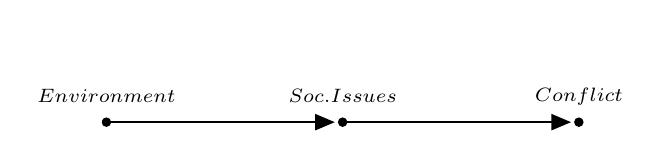
\begin{tikzpicture}[line cap=round,line join=round,>=triangle 45,x=1cm,y=1cm]
\clip(-1,-0.2) rectangle (6.6,1.2);
\draw [->,line width=0.6pt] (0,0) -- (2.9,0);
\draw [->,line width=0.6pt] (3,0) -- (5.9,0);
\begin{scriptsize}
\draw [fill=black] (0,0) circle (1.5pt);
\draw[color=black] (0,0.33) node {$Environment$};
\draw [fill=black] (3,0) circle (1.5pt);
\draw[color=black] (3,0.33) node {$Soc. Issues$};
\draw [fill=black] (6,0) circle (1.5pt);
\draw[color=black] (6,0.33) node {$Conflict$};
\end{scriptsize}
\end{tikzpicture}

or \pause

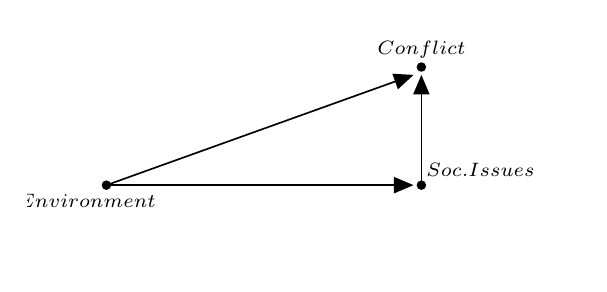
\begin{tikzpicture}[line cap=round,line join=round,>=triangle 45,x=1cm,y=1cm]
\clip(-2,-1) rectangle (5,2);
\draw [->,line width=0.6pt] (-1,0) -- (2.9,0);
\draw [->,line width=0.6pt] (3,0) -- (3,1.4);
\draw [->,line width=0.6pt] (-1,0) -- (2.9, 1.4);
\begin{scriptsize}
\draw [fill=black] (-1,0) circle (1.5pt);
\draw[color=black] (-1.25,-0.2) node {$Environment$};
\draw [fill=black] (3,0) circle (1.5pt);
\draw[color=black] (3.75,0.2) node {$Soc. Issues$};
\draw [fill=black] (3,1.5) circle (1.5pt);
\draw[color=black] (3,1.72) node {$Conflict$};
\end{scriptsize}
\end{tikzpicture}
}

\section{Assignment 2}

\frame{
\frametitle{Assignment 2}
Details:
\begin{itemize}
\item Due in Week 23 \pause
\item 2000 words (or 2500 if in pairs) $\pm 10\%$ \pause
\item Choose \textbf{one} conflict from the UCDP data. \pause Be sure to check if it was ongoing in earlier/subsequent years, and include them if that's the case. \pause \emph{EACH ROW IS A CONFLICT-YEAR}. \pause
\item Explain conflict initiation, continuation, or other dynamics by using the frameworks we've seen in class: \pause
	\begin{itemize}
	\item[--] Terrorism \pause
	\item[--] Grievance \emph{vs} feasibility \pause
	\item[--] Bargaining \pause
	\item[--] Environmental issues \pause
	\item[--] Gender dynamics \pause
	\item[--] Ethnic conflict
	\end{itemize}
\end{itemize}
}

\frame{
\frametitle{Assignment 2: suggestions}
Some suggestions to keep in mind:
\begin{itemize}
\item Always define key concepts before using them. \pause Assume the reader \textbf{does not know} what you're talking about \pause
\item Describe \textbf{AND} explain \pause ($\neq$ what you did for the first assignment, where you mostly only described) \pause
\item Refer to relevant literature from the module outline \pause
\item Keep close to the word count ($\pm 10\%$) \pause
\item Be concise: \pause structure your essay, incorporate and combine sentences, avoid repetition, don't refer back, keep your sentences to 25-30 words and paragraphs 250-300 words \pause
\item No table is required. If you include one, keep it brief and be sure that it serves your assignment
\end{itemize} \pause

Questions?
}

\frame{
\frametitle{Conclusion}
\begin{center}
All clear? More questions? \\
See you next week!
\end{center}
}

\end{document}